\lab{Algorithms}{Principal Component Analysis}{Principal Component Analysis}
\objective{Understand the basics of principal component analysis}

Understanding the variance in complex data is one of the initial tasks in exploratory data analysis. For example, consider the following scatter plot displaying the sepal and petal lengths of 100 different irises.
\begin{figure}[h]
\centering
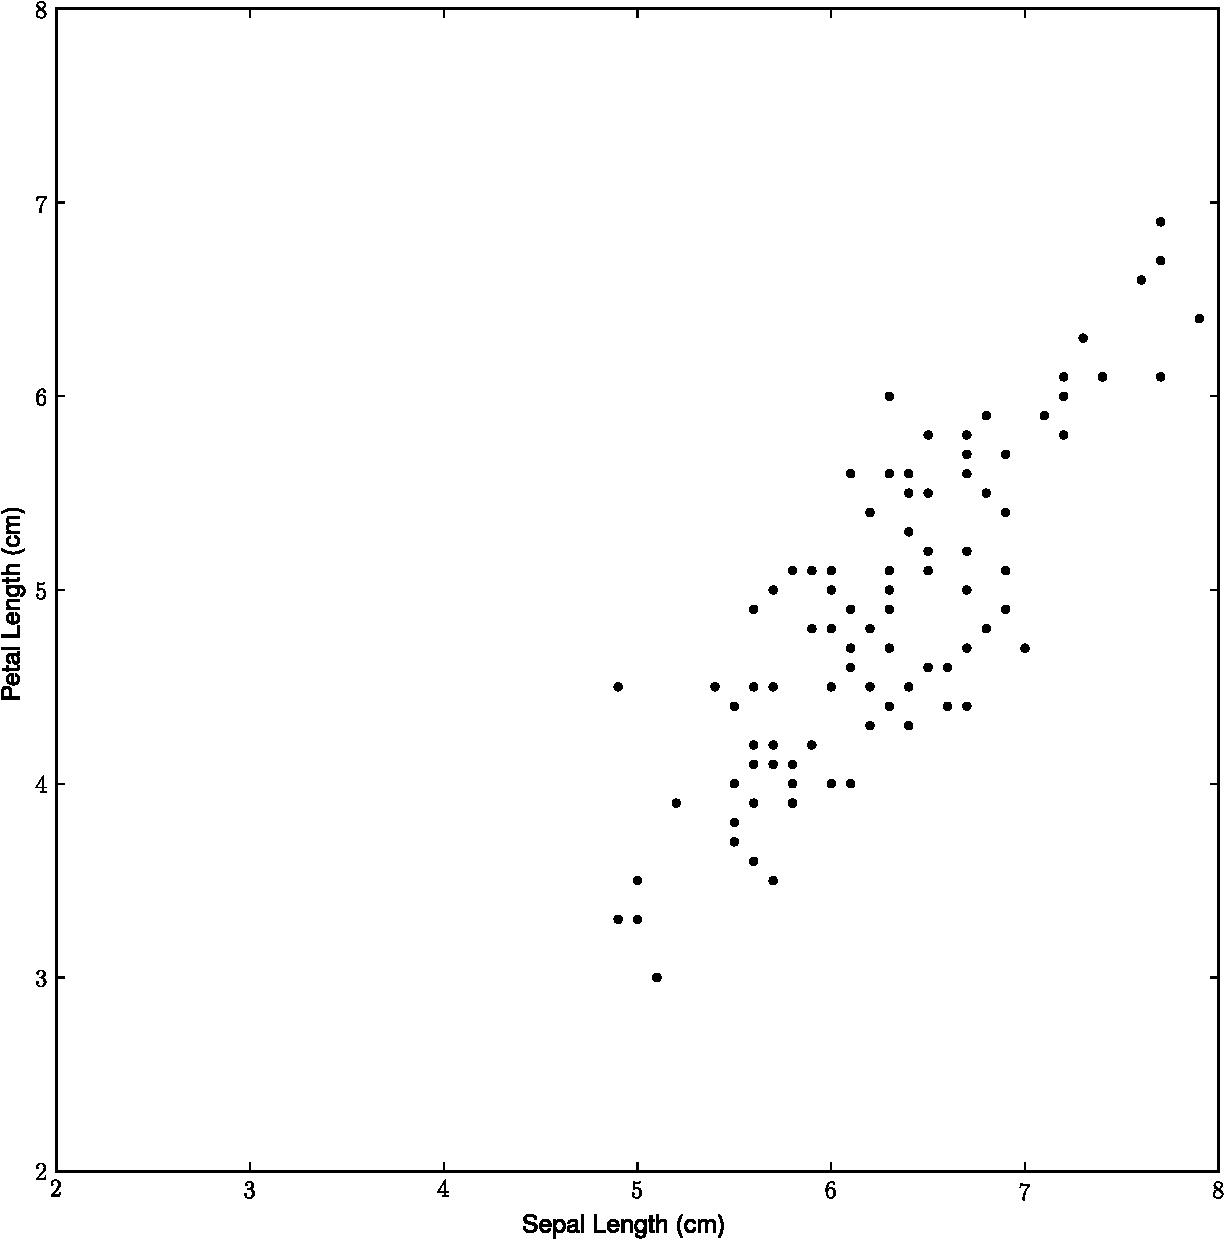
\includegraphics[width=\textwidth]{iris0.pdf}
\end{figure}
Considering this data, we might ask what aspect of irises is most distinguishing (causes the greatest variance). Upon examination, we might see that the petal length ranges between $3$ and $7$ cm, while the sepal length only ranges between $5$ and $8$. So we might be tempted to say that the most distinguishing aspect of irises is their petal length.
But this is only considering the \emph{features} of the data individually, and not collectively. This data is clearly correlated, and a more careful consideration would lead us to conclude that the most distinguishing aspect of irises is their overall size: some irises are just bigger than others.
\begin{figure}[h]
\centering
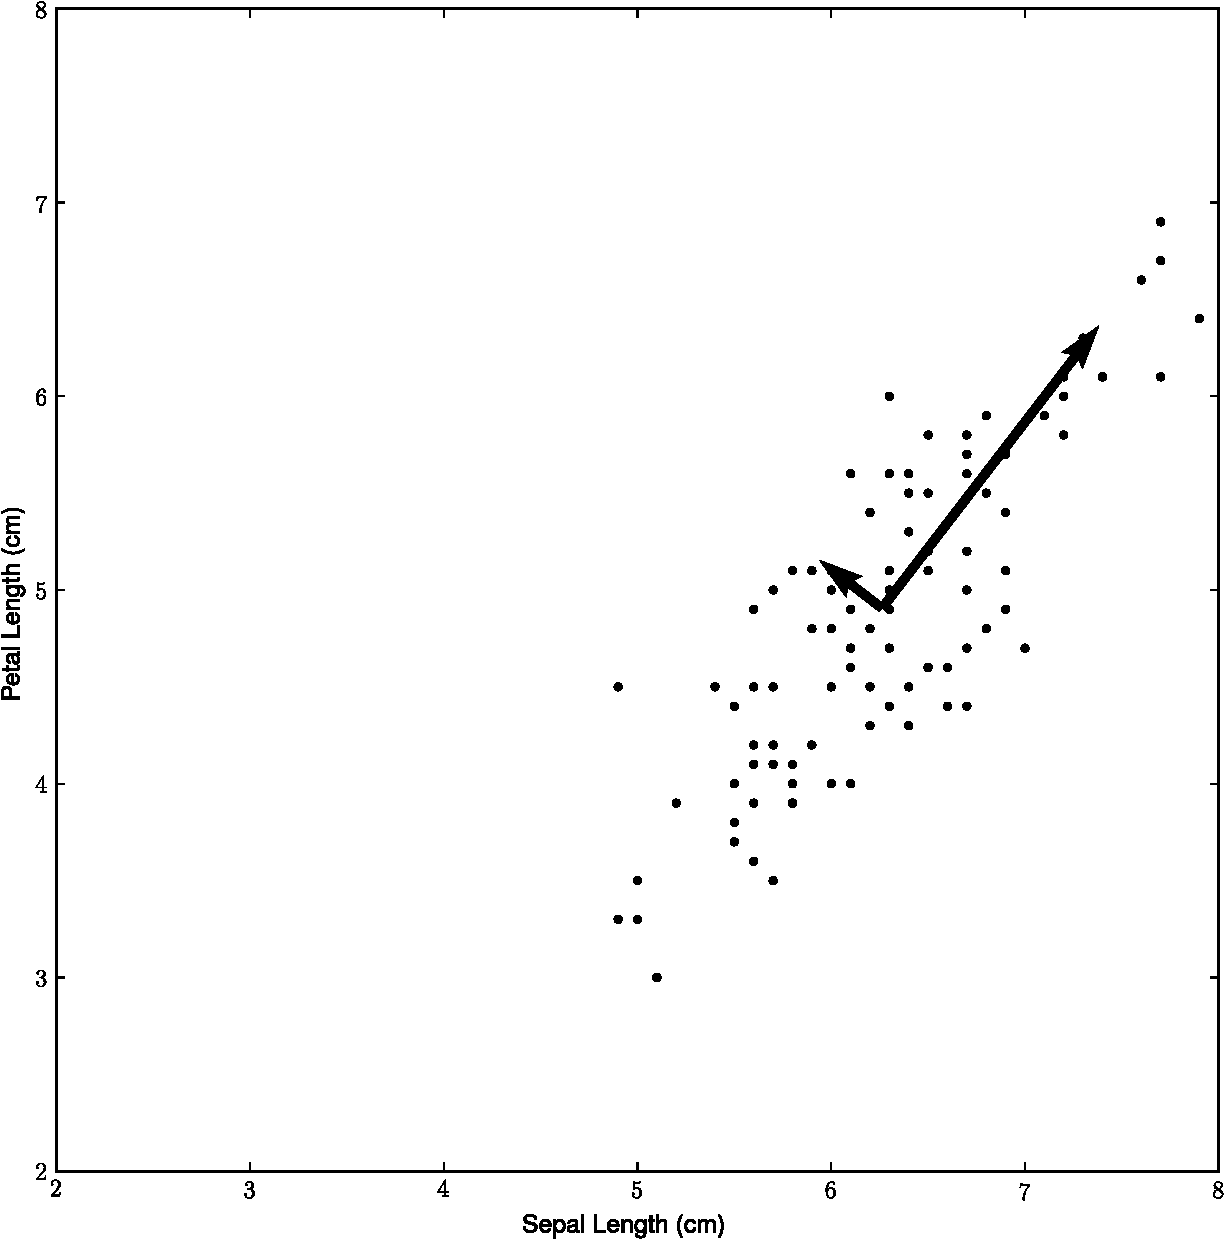
\includegraphics[width=\textwidth]{iris2.pdf}
\end{figure}

Principal Component Analysis (PCA) is a multivariate statistical tool used to orthogonally transform a set of observations over $K$ features into a set of values whose variables are linearly uncorrelated. More specifically, the first new variable will account for the greatest variance in the set of observations, the second variable will be orthogonal to the first, accounting for the second greatest variance in the set of observations, etc. These variables are called the \emph{principal components} and are all orthogonal (uncorrelated) to each other. The first several principal components capture most of the variance in the observation set, and hence provide a great deal of information about the data.
In our example above, the first principal component was \[\left[ \begin{array}{cc} 0.61 & 0.79 \end{array} \right] \]  and the second was \[\left[ \begin{array}{cc} -0.79 & 0.61 \end{array} \right] \] respectively accounting for $92\%$ and $8\%$ of the variance in the data. The first principal component is the vector along which the greatest variance in the observations occurs, and the second component is the vector along which the remaining variance occurs, orthogonal to the first. PCA is used to identify these principal components, and then transform the observations from the original feature space to the principal component space.
PCA is more useful with observations over a large feature space (high dimensionality). It can be used to reduce the dimensionality of the feature space while simultaneously capturing most of the observation variance in a few dimensions.

Throughout we will use the iris data set, which can be obtained as follows:
\begin{lstlisting}
: import sklearn.datasets as datasets;
: iris = datasets.load_iris()
\end{lstlisting}
We will represent the observations as $X$, where each observation is a row, and each column is a specific feature. Generally, the observations are first translated to be centered at the origin. At this point, the data is often scaled to remove discrepancies arising from different units of measure (i.e. centimeters vs meters), and we call the centered and scaled data $Y$. In this lab and the next, we will not have any scaling issues, so we won't address this further. 

We next find the truncated SVD of our centered and scaled data, $$Y = U\Sigma V^{H}$$ where the nonzero entries of $\Sigma$ are the square roots of the nonzero eigenvalues of $Y^{H}Y$. The columns of V are the principal components, and the corresponding eigenvalues provide us information about how much variance is captured in each principal component. More specifically, let $\lambda_{i}$ be the square of the $i^{th}$ non-zero singular value. Then the value $$\frac{\lambda_{i}}{\sum_{j=1}^{K} \lambda_{j}}$$ is the percentage of the variance captured by the $i^{th}$ principal component.

In general, we are only interested with the first several principal components, leaving us wondering how many principal components we should keep. There are a number of ways to decide this. One is to only keep the first two principal components, as these enable us to project the data into $2$-dimensional space, which is easy to visualize. Another way is to only keep the set of principal components accounting for a certain percentage (say $80\%$) of the variance. A third method is to examine the scree plot of the percentage of variance captured by each principal component, as in Figure \ref{fig:scree}.
\begin{figure}
\centering
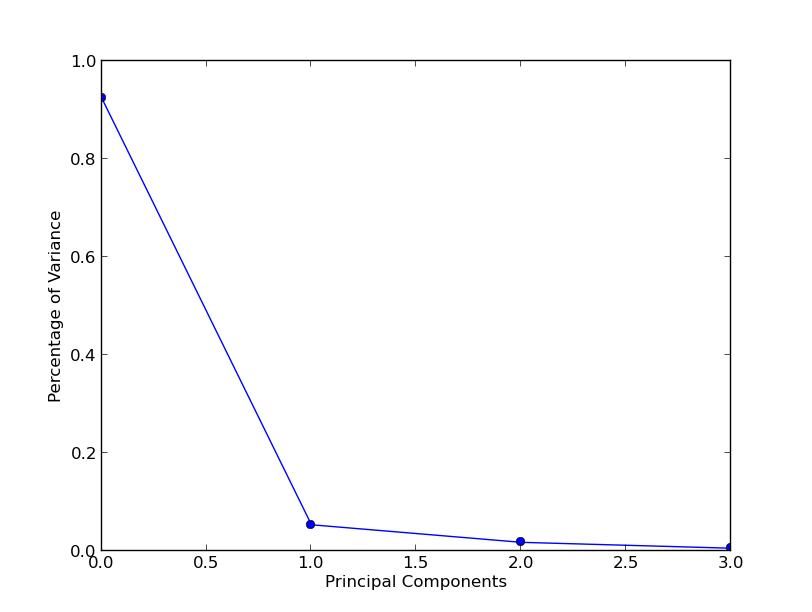
\includegraphics[width=\textwidth]{scree.jpg}
\caption{Scree plot of the percentage of variance for PCA on the iris dataset}
\label{fig:scree}
\end{figure}
Upon examination, we see that there is a distinct change after the first principal component. This method is referred to as finding the "elbow" of the scree plot, in which case we consider all the principal components on the left of the elbow. In this case, that is simply the first principal component, which accounts for $92\%$ of the variance.
We can transform the observations from the original feature space by computing 
\begin{equation*}
\widehat{X} = U\Sigma
\end{equation*}
where $U$ and $\Sigma$ are from the truncated SVD found previously. We can then represent $\widehat{X}$ well by only keeping the first $K$ columns, where $K$ is the number of principal components retained. In this way, we have transformed our observations from the original feature space into an orthoganalized space, where the first several components explain most of the variance in the observations, allowing us to further reduce the dimensionality in a reasonable way.

In Figure \ref{fig:irispca} we display the transformed iris data set, plotting the first principal component against the second. We can see that this reduction helps us to see the distinctions between the three different species, using only two dimensions instead of the full four dimensions of the feature space.
\begin{figure}
\centering
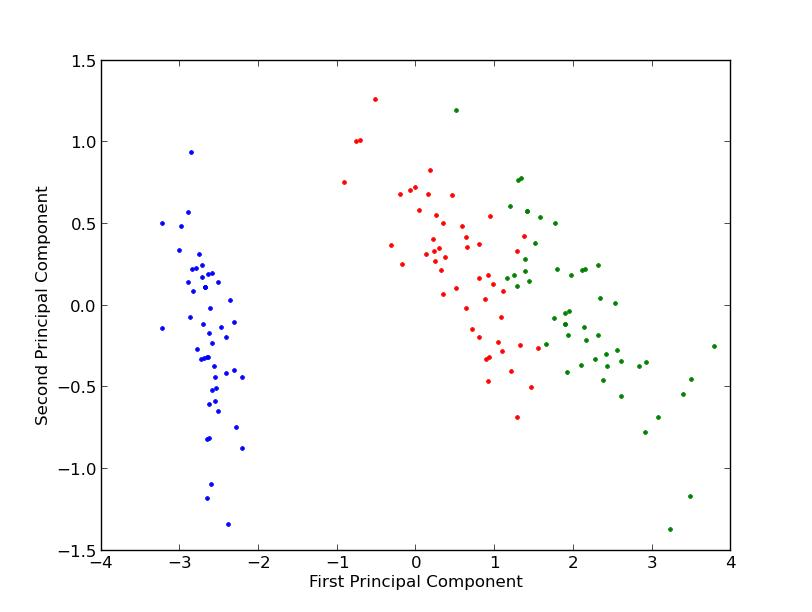
\includegraphics[width=\textwidth]{irispca.jpg}
\caption{Plot of transformed iris data, keeping only the first two principal components. Blue - Setosa, Red - Versicolor, Green - Virginica}
\label{fig:irispca}
\end{figure}

\begin{problem}
Write a function to perform PCA on an arbitrary data set with real-valued features. Your function should take as arguments the dataset as an array, a boolean value to determine whether or not to center the data, and a percentage used to determine the number of principal components to retain. It should return a vector of the percentage of the variance explained by each principal component, the retained principal components, and the transformed, truncated data.
\end{problem}

\begin{problem}
Test your PCA function on the iris data set, retaining two principal components. Plot the transformed, truncated data, coloring each species differently.
\end{problem}

\begin{problem}
Make a scree plot of the percentage of variance captured by each principal component for the iris data set.
\end{problem}